% Imported from datasets/recipes/audio-video-production/README.md
\chapter{M11 训练数据的制作与隔离}\label{seedance-m11}
\moduleinfo{M11}{基础方法与机制解释}{\hyperref[src-seedance-1.0]{\texttt{seedance-1.0}}、\hyperref[src-tarsier2]{\texttt{tarsier2}}、\hyperref[src-phantom]{\texttt{phantom}}、\hyperref[src-vincie]{\texttt{vincie}}、\hyperref[src-long-context-tuning]{\texttt{long-context-tuning}}、\hyperref[src-tarsier-code]{\texttt{tarsier-code}}、\hyperref[src-diffsynth-code]{\texttt{diffsynth-code}}、\hyperref[src-vincie-code]{\texttt{vincie-code}}}


视频训练数据不是一个``视频文件加一句描述''的目录。参考控制需要知道素材属于哪个主体，局部编辑需要知道允许改变的范围，续写需要知道哪些帧已经发生。数据制作的目标，是把这些约束变成可重复执行、可追踪来源的样本。

\section{先定义样本，再决定收什么}\label{seedance-m11-ux5148ux5b9aux4e49ux6837ux672cux518dux51b3ux5b9aux6536ux4ec0ux4e48}

一个训练样本应围绕一个目标任务组织，包含目标片段、条件、文字描述、参考绑定和有效监督位置。原始长视频、场景和主体属于上层来源信息，可以派生多个样本，但不能在拆分后丢失它们的关联。

{\def\LTcaptype{table} % do not increment counter
\small\setlength{\tabcolsep}{3pt}\renewcommand{\arraystretch}{1.18}
\begin{longtable}[]{@{}
  >{\raggedright\arraybackslash}p{(\linewidth - 4\tabcolsep) * \real{0.1900}}
  >{\raggedright\arraybackslash}p{(\linewidth - 4\tabcolsep) * \real{0.3900}}
  >{\raggedright\arraybackslash}p{(\linewidth - 4\tabcolsep) * \real{0.4200}}@{}}
\toprule\noalign{}
\begin{minipage}[b]{\linewidth}\raggedright
任务
\end{minipage} & \begin{minipage}[b]{\linewidth}\raggedright
条件
\end{minipage} & \begin{minipage}[b]{\linewidth}\raggedright
目标与关键标签
\end{minipage} \\
\midrule\noalign{}
\endhead
\bottomrule\noalign{}
\endlastfoot
文本生成视频 & 动作与场景描述 & 目标片段、事件顺序 \\
主体参考 & 参考图与动作要求 & 同主体目标、角色绑定、允许变化属性 \\
局部编辑 & 源片段、指令、时间与空间 mask & 编辑后片段、保持项与变化项 \\
续写 & 历史片段、新事件要求 & 后续片段、历史截止时间 \\
\end{longtable}
}

如果评测未见身份，训练与测试需要身份隔离；如果只评同身份的新场景，则应按场景和原始来源隔离。二者回答不同问题，不能混成一个泛化结论。

\section{原始素材入库需要保留什么}\label{seedance-m11-ux539fux59cbux7d20ux6750ux5165ux5e93ux9700ux8981ux4fddux7559ux4ec0ux4e48}

每份媒体保存内容哈希、来源、版本、训练与再分发使用范围，以及容器、codec、分辨率、帧率和时间戳信息。参考素材、编辑源和目标媒体应各有记录，不能只批准目标文件。

视频还可能包含旋转、HDR 色彩、可变帧率和音频偏移。预处理必须保存这些信息及对应变换：真正重采样音频，真正调整视频帧序列，并保留原时间戳到新帧索引的映射。缓存可按``原文件哈希、变换配置、工具版本''确定，任何一项改变都产生新版本。

\section{切镜、过滤与去重怎样衔接}\label{seedance-m11-ux5207ux955cux8fc7ux6ee4ux4e0eux53bbux91cdux600eux6837ux8854ux63a5}

自然切镜检测适合把长视频拆成可处理片段，但闪光、快速运动和淡入淡出容易误判，必须抽检。质量标签应分别记录压缩损伤、失焦、遮挡字幕、过暗、静止、异常加速和声画错位，避免一个总分掩盖可修复的问题。

\begin{figure}
\centering
\pandocbounded{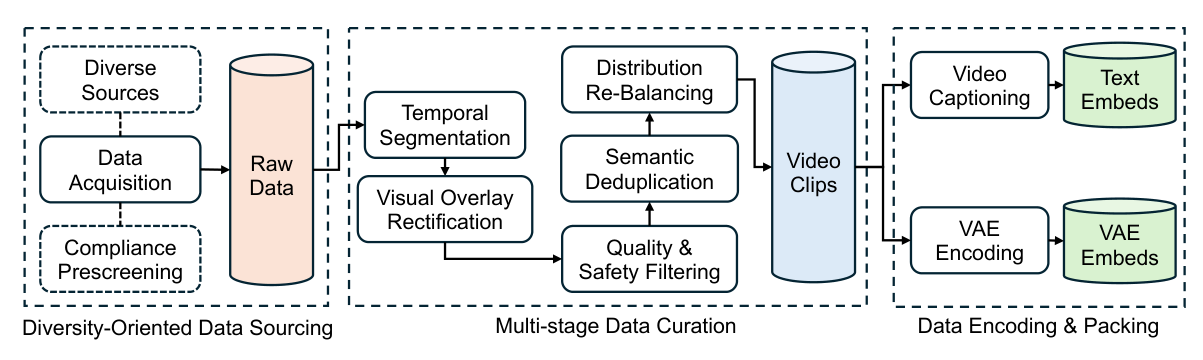
\includegraphics[keepaspectratio,alt={从多来源视频整理到描述与潜变量打包 （论文示意，来源：seedance-1.0）}]{assets/seedance/figures/data-pipeline.png}}
\caption{从多来源视频整理到描述与潜变量打包 （论文示意，来源：seedance-1.0）}
\end{figure}

缩放、裁剪和补帧时，框、mask、关键点与相机条件必须同步变换。如果模型要求 \(F=1+4k\)，补出的帧需要有效位标记，不能让它们像真实帧一样计入损失。

去重至少包含文件哈希、跨编码近重复和内容聚类。相邻镜头、同原片不同剪辑、共享参考和同主体关系会形成来源图；需要按关联分组划分训练、验证、测试，不能只随机打散 shot。

分布平衡也应在划分后处理：训练集可以提高长尾动作采样率，测试集则保留预先定义的分布。不断看测试结果再调采样或阈值，会让测试失去独立性。

\section{Caption 的工作是描述事实}\label{seedance-m11-caption-ux7684ux5de5ux4f5cux662fux63cfux8ff0ux4e8bux5b9e}

好的视频描述同时包含静态属性与动态事件：主体外观、环境、动作、物体状态、相机和可观测光照。事件应附时间范围，多镜头还要区分全局角色信息与镜头局部变化。

描述模型可以先由人工细粒度标注训练，再扩大自动描述规模。Tarsier2 采用 Qwen2-VL 初始化，并结合时间 grounding 和描述偏好优化；使用它做生成数据标注时，仍需检查是否漏事件、错顺序或编造动作。基础描述模型全参训练，与某个下游任务冻结视觉编码器，是两种不同设置。

Prompt 改写与 caption 生成也不同：前者把用户要求变成可用指令，后者从媒体提取事实。两者可以使用相近的结构，但改写器不能把``猫''改成``狗''，caption 模型也不能猜测画外台词和人物动机。

\section{参考、编辑与续写各有什么泄漏风险}\label{seedance-m11-ux53c2ux8003ux7f16ux8f91ux4e0eux7eedux5199ux5404ux6709ux4ec0ux4e48ux6cc4ux6f0fux98ceux9669}

主体参考若直接从目标帧截取，模型容易复制背景和姿态。跨片段同主体配对更适合学习身份保持，但相似特征并不证明身份相同，需要标签或人工核实。

编辑样本可以来自受控三维重渲染、真实人工编辑对或视频变化挖掘。前两类更容易提供明确真值，第三类应标为弱监督。相机、遮挡和光照一起变化时，不能只给一个``换颜色''标签。

续写样本必须记录历史截止时间，目标未来帧不得混入历史参考。已生成的训练轨迹也应与真实历史区分，因为模型在自生成历史上面对的误差分布不同。

\section{人工抽检怎样带动自动化}\label{seedance-m11-ux4ebaux5de5ux62bdux68c0ux600eux6837ux5e26ux52a8ux81eaux52a8ux5316}

可以先制作约 200 条分层试样，覆盖任务、运动幅度和主体数，并对至少一部分进行双人独立标注。这个数量是流程起点，不是充分数据规模。先建立争议样例的裁定规则，再扩大自动生成。

抽检分别统计事实准确率、关键事件召回、身份配对正确率、mask 越界和时间偏差。错误率高的类别增加抽样，已经稳定的类别才逐步降低人工比例。自动分数阈值需要用真实样本校准，不能从另一个数据集直接复制。

\section{编码与打包怎样支持重做}\label{seedance-m11-ux7f16ux7801ux4e0eux6253ux5305ux600eux6837ux652fux6301ux91cdux505a}

VAE 和文本编码器固定后，可以离线缓存潜变量与文本特征，但必须记录模型哈希、shape、dtype、缩放、后验采样方式和预处理。裁剪改变后复用旧 latent，会让媒体和条件悄悄错位。

按形状或 token 预算分桶可减少 padding。多个场景打包时，attention 应在场景边界隔离；缺音频、无效 padding、已知条件和生成目标分别设置有效位。

最终 manifest 保存每阶段输入、通过和淘汰数量，原因分布、split、来源分组、标注和变换版本。若一份素材撤回，应能追踪其派生 caption、latent、偏好对和训练运行。schema 校验可以发现字段、时间和已登记来源的冲突，媒体真实性、授权有效性与标注质量仍需真实处理与人工核查。

\section{真实工程从哪里进入}\label{seedance-m11-ux771fux5b9eux5de5ux7a0bux4eceux54eaux91ccux8fdbux5165}

批量描述入口可直接读 \href{https://github.com/bytedance/tarsier/blob/63de87a760c2aec6b31470a08046969a13787126/tasks/inference_caption.py}{Tarsier caption} 和 \href{https://github.com/bytedance/tarsier/blob/63de87a760c2aec6b31470a08046969a13787126/scripts/run_inference_caption.sh}{启动脚本}；训练数据如何进入模型可读 \href{https://github.com/modelscope/DiffSynth-Studio/blob/d32f72424cd22bc0ea8100cc57559149b4eac933/examples/wanvideo/model_training/train.py}{DiffSynth WanTrainingModule}。参考/编辑数据字段仍需按具体任务制作，不能把一个通用 caption CSV 自动解释为身份或局部保持监督。
